\section{\ourslong}
\label{sec:method}
In this section, we start by analyzing ViT outputs to motivate our approach (\S\ref{sec:factorization}). Then, we introduce our per-image denoising method, which removes artifacts and produces noise-free features (\S\ref{sec:per_img_denoising}). Lastly, we explain how the noise-free features are utilized as pseudo-labels to train a generalizable denoiser (\S\ref{sec:gen_denoiser}). Our method pipeline is depicted in \cref{fig:method}.

%##################################################################################################
\begin{figure}[t!]
    \centering
    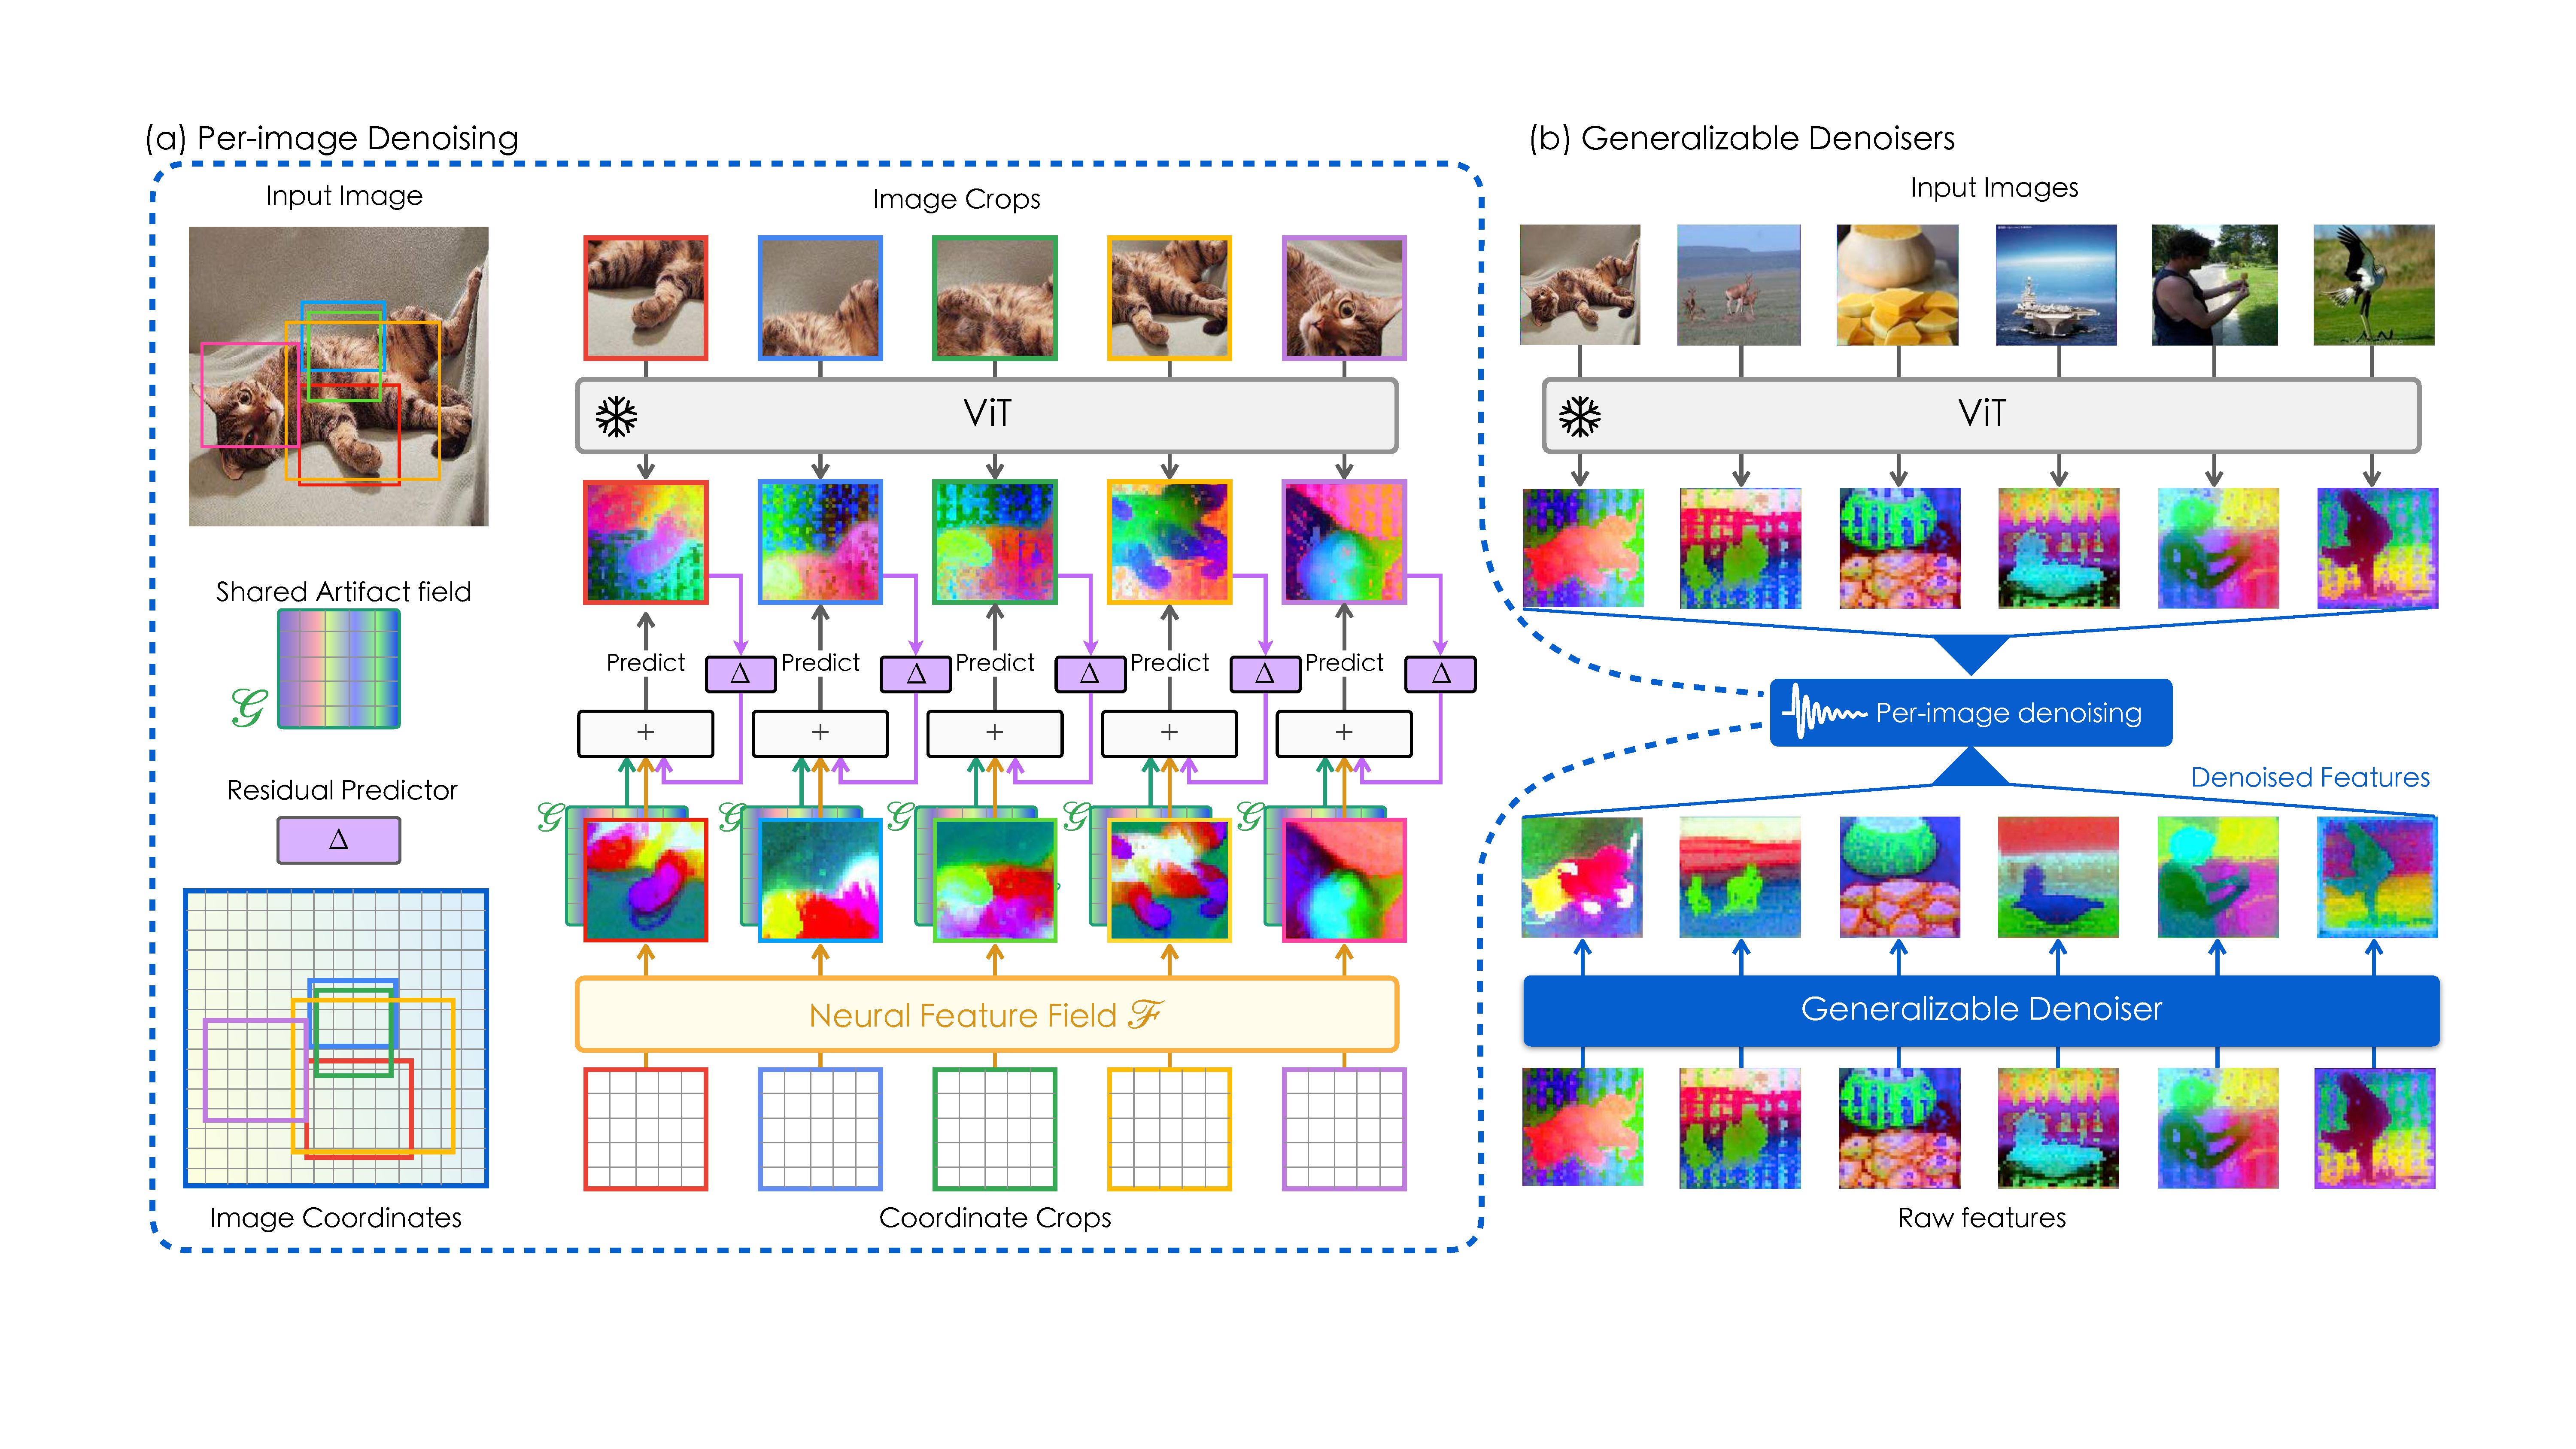
\includegraphics[width=1\linewidth]{figures/fig4_method_overview.pdf}
    \caption{\textbf{Method Overview.} \ours consists of a two-stage denoising pipeline. (a) In the first stage, our method decomposes the raw feature of an image crop into a noise-free semantics term $\mathcal{F}$, an input-independent, position-related artifact term $\mathcal{G}$, and an additional residual term $\Delta$. (b) In the second stage, we train a generalizable denoiser to predict clean features from their original features. At inference time, only a single feedforward is needed to obtain denoised features.}
    \label{fig:method}
\end{figure}
%##################################################################################################



\subsection{Factorizing ViT Outputs}
\label{sec:factorization}
Our method is grounded in the principle that ideal visual features should be inherently translation and reflection invariant, \ie, the features of an object should remain consistent, regardless of changes in the viewing window, size, and orientation. However, as indicated in \cref{eq1,eq2,eq3,eq4} and \cref{fig:vit_arch}-(b), ViTs intermix patch embeddings with positional embeddings, thereby breaking the transformation invariance of visual features. This breach of invariance might not appear immediately problematic, but our investigations, illustrated in \cref{fig:vit_arch}-(a) and (c), reveal a distinct correlation between the inclusion of positional embeddings and the emergence of undesirable artifacts in ViT outputs. Particularly, the middle row of \cref{fig:vit_arch}-(c) shows that these artifacts persist with minor variation across different images, highlighting their consistency independent of the input content.

These observations motivate us to decompose ViT outputs into three terms: (1) an input-dependent, noise-free semantics term $f(\vb{x})$\footnote{Throughout this paper, we use ``noise'' and ``artifact'' interchangeably.}; (2) an input-independent artifact term related to spatial positions $g(\vb{E}_{pos})$; (3) and a residual term that accounts for the interdependence of semantics and positions  $h(\vb{x}, \vb{E}_{pos})$. The decomposition is formally expressed as:
\begin{equation}
    \mathrm{ViT}(\vb{x}) \approx f(\vb{x}) + g(\vb{E}_{pos}) + h(\vb{x}, \vb{E}_{pos}) \label{eq:decomposition}
\end{equation}

This factorization is universally applicable to all ViTs. For example, in scenarios where the output feature map is spatially invariant (\eg, no positional embedding is used), the sum of $g$ and $h$ becomes a constant bias term that can be merged into $f$.


\subsection{Per-image Denoising with Neural Fields}
\label{sec:per_img_denoising}
Directly addressing the above decomposition problem within a single forward pass in a ViT is impractical due to the intertwined nature of output features. To overcome this, we exploit the consistencies in cross-view features and artifacts: (1) \textit{Feature consistency} refers to the transformation invariance of visual features, where despite the varied spatial transformations, the semantic content remains invariant; (2) \textit{Artifact consistency} means that the input-independent artifact remains observable and constant across all transformations. Formally, consider an image $\vb{x}$ and a set of its randomly transformed views $T(\vb{x})=\{t_0(\vb{x}), t_1(\vb{x}), \cdots\}$, where each transformation $t_{i}$ is drawn from a distribution of random augmentations $\mathcal{T}$, consisting of random resizing, cropping, and flipping. Our goal is to derive a mapping $f$ such that the semantic features obtained from any transformed view, $f\left(t\left(\vb{x}\right)\right)$, are equivalent to the transformed original semantic features, $t\left(f(\vb{x})\right)$; that is, $f\left(t\left(\vb{x}\right)\right)=t\left(f(\vb{x})\right)$ with $t \sim \mathcal{T}$. Next, we describe our approach for learning the different terms in \cref{eq:decomposition} in conjunction to derive $f$.

\paragraph{Neural fields as feature mappings.} At the core of our approach is to have a holistic image semantics representation $\mathcal{F}$, for \textit{each individual image}, alongside a spatial artifact feature representation, $\mathcal{G}$, shared by \textit{all transformed views}. The holistic image feature representation $\mathcal{F}$ is designed to capture spatially independent, artifact-free semantics, while $\mathcal{G}$ should encode position-dependent but input-independent noise. We use coordinate networks, known as neural fields \cite{tancik2020fourfeat,muller2022instant,shen2023distilled,kobayashi2022decomposing,kerr2023lerf,yang2023emernerf}, to actualize $\mathcal{F}$ and $\mathcal{G}$. Specifically, we define $f(t(\vb{x}))=\mathcal{F}(\mathrm{coords}(t(\vb{x})))$, where $\mathrm{coords}(\cdot)$ extracts the pixel coordinates of the transformed views relative to the original image $\vb{x}$, and $g(\vb{E}^{i}_{pos})=\mathcal{G}(i)$, with $i \in \{0, \cdots, N-1\}$ denoting the patch index. For simplicity, we use $\mathcal{G}$ to denote the 2D artifact feature map reshaped from the 1D ordered sequence $\{\mathcal{G}(i)\}_{i=0}^{N-1}$. We refer to $\mathcal{F}$ and $\mathcal{G}$ as the semantics field and the artifact field, respectively.

\paragraph{Learning the decomposition.} We learn the semantics field $\mathcal{F}$, the artifact field $\mathcal{G}$, and the residual term $\Delta$ by minimizing a regularized reconstruction loss:
\begin{align}
    \mathcal{L}_\text{recon}      & = \mathcal{L}_{\text{distance}} + \alpha \mathcal{L}_{\text{residual}} + \beta  \mathcal{L}_{\text{sparsity}} \label{eq:recon}                             \\
    \mathcal{L}_{\text{distance}} & = 1 - \cos(\vb{y}, \widehat{\vb{y}}) + \| \vb{y} - \widehat{\vb{y}} \|_2,                                                                                  \\
    \mathcal{L}_\text{residual}   & = \|\mathrm{sg}\left(\vb{y} - \widehat{\vb{y}'}\right) - \widehat{\Delta}\|_2, \hspace{1em} \mathcal{L}_{\text{sparsity}} = \|\widehat{\Delta}\|_1         \\
    \text{where}~~\vb{y}          & = \mathrm{sg}\left(\mathrm{ViT}\left(t\left(\vb{x}\right)\right)\right), \hspace{2em} \widehat{\vb{y}} = \widehat{\vb{y}'} + \mathrm{sg}(\widehat{\Delta}) \\
    \widehat{\vb{y}'}             & = \mathcal{F}_{\theta}(\mathrm{coords}(t(\vb{x}))) + \mathcal{G}_{\xi}, \hspace{0.6em} \widehat{\Delta} = h_{\psi}(\vb{y})
\end{align}
Here, $\cos(\cdot, \cdot)$ denotes the cosine similarity, $\mathrm{sg}(\cdot)$ represents the stop-gradient operation, $t(\cdot)$ is a random transformation sampled from $\mathcal{T}$, and $\theta$, $\xi$ and $\psi$ are the learnable parameters. Our loss function is designed to encourage $\widehat{\Delta}$ to remain minimal by imposing a sparsity regularization, thereby allowing $\widehat{\vb{y}'}$ to represent as much of the ViT output as possible. The use of stop-gradient operators is to avoid trivial solutions, such as identity mapping. The reconstructed feature from our method is $\widehat{\vb{y}} = \mathcal{F}_{\theta}\left(\mathrm{coords}\left(t\left(\vb{x}\right)\right)\right) + \mathcal{G}_{\xi} + \mathrm{sg}\left(h_{\psi}\left(\mathrm{ViT}\left(t\left(\vb{x}\right)\right)\right)\right)$, each term corresponding to $f, g$, and $h$ as defined in \cref{eq:decomposition}.



\paragraph{Optimization.} We break our optimization process into two phases, each spanning half of the total training iterations. In the first phase, we train $\mathcal{F}_\theta$ and $\mathcal{G}_{\xi}$ using only $\mathcal{L}_{\text{distance}}$, allowing them to capture a significant portion of the ViT outputs. After completing half of the optimization iterations, we freeze $\mathcal{G}_\xi$ and continue to train $\mathcal{F}_\theta$ alongside $h_\psi$ using $\mathcal{L}_\text{recon}$ for the rest iterations. The coefficients $\alpha$ and $\beta$ in $\mathcal{L}_\text{recon}$ balance loss scales and regulate the residual term to prevent $\widehat{\Delta}$ from over-explaining the outputs.

\subsection{Generalizable Denoiser}
\label{sec:gen_denoiser}
Our per-image denoising method can already effectively remove artifacts from ViT outputs, yielding visually stunning denoised feature maps. The problems we are left with are run-time efficiency and distribution shifts. Specifically, the per-image denoising process is suitable for offline applications but undesired for real-time applications, and individually denoised feature maps can lead to feature distribution shifts due to sample bias, which hampers the feature coherence across images. To address these issues, we introduce a generalizable denoiser.

After applying per-image denoising, we accumulate a dataset of pairs consisting of noisy ViT outputs $\vb{y}$ and their denoised counterparts $\mathcal{F}$, denoted as $\mathcal{B}=\{\left(\vb{y}_i, \mathcal{F}_i\right)\}_{i=1}^B$. We then train a denoiser network  ${D}_\zeta$ to predict noise-free features from raw ViT outputs, \ie, $\hat{\mathcal{F}} = D_\zeta(\vb{y})$. The loss function is:
\begin{align}
    \mathcal{L}_{\text{distance}}^\text{\ours} & = 1 - \cos\left(D_\zeta\left(\vb{y}\right), \mathcal{F}\right) + \|D_\zeta\left(\vb{y}\right) - \mathcal{F} \|_2 \label{eq:gen_loss}
\end{align}
Our generalizable denoiser is implemented as a single Transformer block, supplemented with additional learnable positional embeddings that are applied post the forward pass of a ViT. This design aims to mitigate the input-independent artifacts. To predict denoised features, the outputs from a pre-trained ViT are added with these positional embeddings and then processed through the Transformer block.

Notably, this learned denoiser is lightweight, thus adding negligible latency to the original ViT and facilitating real-time applications. It also learns to generalize across samples, mitigating the distribution shift issue in the per-image denoising process.



